\section{Results}
\label{sec:eval}

\subsection{Input Graph Characteristics}

\begin{figure}
	\centering
	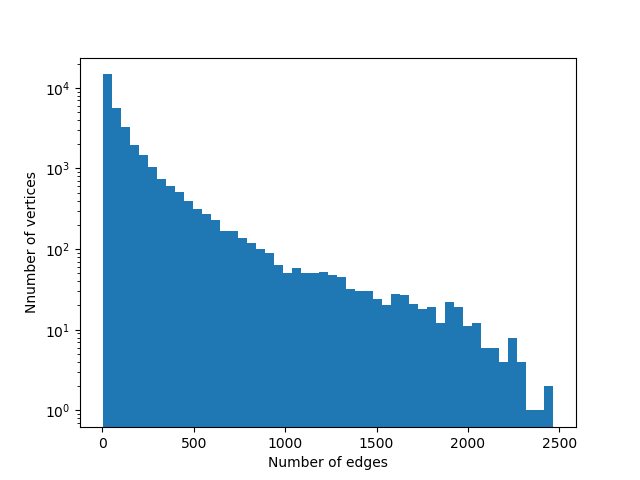
\includegraphics[width=\columnwidth]{../good_plots/degree_distribution_10_mil.png}
	\caption{Degree distribution for a representative graph in our dataset, 
		demonstrating that the graphs we chose are power-law graphs.}
	\label{fig:degree_distribution}
\end{figure}

We selected eleven graphs to analyze. Although we originally chose several 
others, we were limited by the hardware we had the funds to rent to analyzing 
relatively small graphs. A tradeoff exists between the size of a graph, the 
number of workers assigned to handle its vertices, and the amount of memory on 
a server. First, there is a minimum amount of memory that a Giraph worker 
requires in 
order to run. This puts an upper bound on the number of workers that can be run 
on any machine. Second, there appears to be a minimum number of workers that 
can be assigned to a graph of a given size in Giraph: when too few are 
assigned, the job fails. Presumably, this is because each worker can only 
feasibly handle a certain number of vertices, although it is unclear why Giraph 
chooses to terminate jobs rather than allowing them to eventually complete. 
This factor puts a lower bound on the number of workers that can be assigned to 
a graph, which is dependent on the size of the graph. Given these constraints, 
we restricted ourselves to graphs with approximately 200 million edges or fewer.

Our graphs came from the Laboratory for Web Algorithmics (LAW)
\cite{BoVWFI, BRSLLP}. We considered using artificial graphs generated by 
Facebook's Darwini project \cite{edunov_darwini:_2016}, but eventually 
concluded that they were too large. The LAW graphs come 
from a variety of places. We selected a diverse subset of them, as shown in 
Table \ref{tab:graph_types}.

\begin{table*}[t]
	\centering
	\begin{tabular}{r|cccl}
		\textbf{Name} & \textbf{Vertices} & \textbf{Edges} & \textbf{Vertex 
		means...} & \textbf{Edge means...}\\
		\hline
		cnr-2000 & 325557 & 3216152 & Website & Hyperlink\\
		dblp-2011 & 986324 & 6707236 & Scientist & Paper collaboration \\
		enron & 69244 & 276143 & Person & Recipient of email\\
		wordassociation-2011 & 10617 & 72172 & Word & Interpreted association \\
		hollywood-2011 & 2180759 & 228985632 & Actor & Appearance in movie\\
		hollywood-2009 & 1139905 & 113891327 & Actor & Appearance in movie\\
		ljournal-2008 & 5363260 & 79023142 & User & Friend\\
		uk-2007-05@1000000 & 1000000 & 41247159 & Website & Hyperlink\\
		twitter & 41652230 & 1468365182 & User & Follower\\
		uk-2002 & 18520486 & 298113762 & Website & Hyperlink\\
	\end{tabular}
	\caption{Details of graph datasets}
	\label{tab:graph_types}
\end{table*}

We also paid attention to the distribution of the degrees of the vertices in 
the graphs that we chose. Since most natural graphs are power-law distributed, 
our graphs primarily follow that pattern. Figure \ref{fig:degree_distribution} 
shows a representative example of the degree distribution of a graph in our 
dataset. 

\begin{figure}
	\centering
	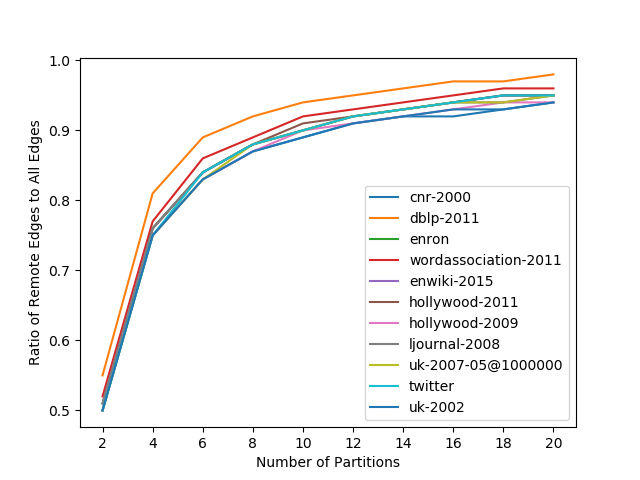
\includegraphics[width=\columnwidth]{../good_plots/remote_to_all_modulo.png}
	\caption{Ratio of remote edges (requiring messages to be sent across the 
	network) to all edges for various numbers of partitions, where partitioning 
	is done by taking the modulus of the vertex ID and number of workers.}
	\label{fig:remote_to_all_mod}
\end{figure}

\begin{figure}
	\centering
	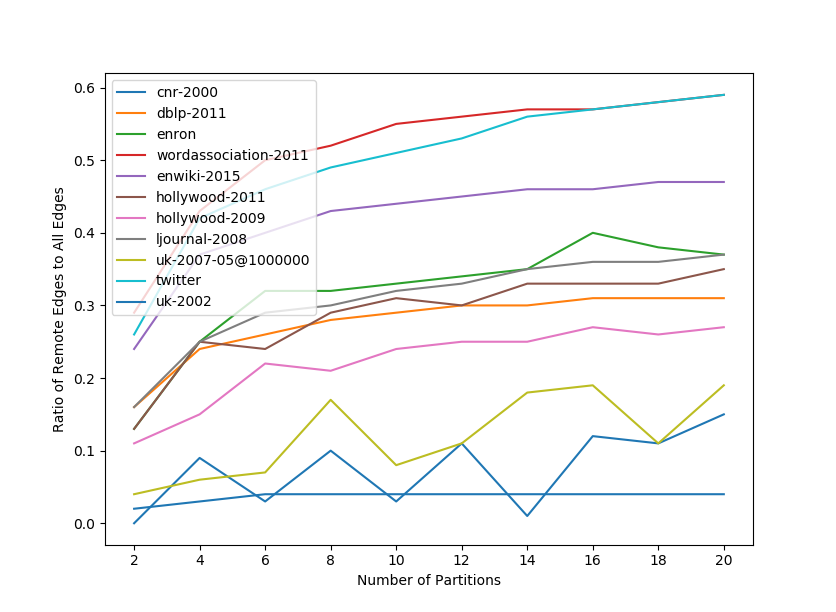
\includegraphics[width=\columnwidth]{../good_plots/remote_to_all_chunked.png}
	\caption{Ratio of remote edges to all edges for various numbers of 
		partitions, where partitioning is done by segmenting the vertex IDs 
		into 
		approximately equal groups.}
	\label{fig:remote_to_all_range}
\end{figure}

We ran experiments to look at two metrics that we believe are predictors of 
performance: the number of edges given to each worker that require network 
requests, and the range of the number of edges given to each worker. We chose 
the first metric because we predict that if a worker is assigned a high 
proportion of edges that require it to make network requests, the time taken to 
run each step of computation will be much higher. Recall that in PageRank, 
every computational step requires a message to be sent along every edge. If 
that message begins and ends at vertices that are stored on the same machine, 
the overhead is much lower than it would be if the source and destination 
vertices are stored on two separate machines, thus necessitating a network 
request. Therefore, we measure the ratio between the number of local edges and 
the total edges assigned to a worker for various numbers of partitions and two 
partitioning schemes. Figures \ref{fig:remote_to_all_mod} and 
\ref{fig:remote_to_all_range} show the results.

\begin{figure}
	\centering
	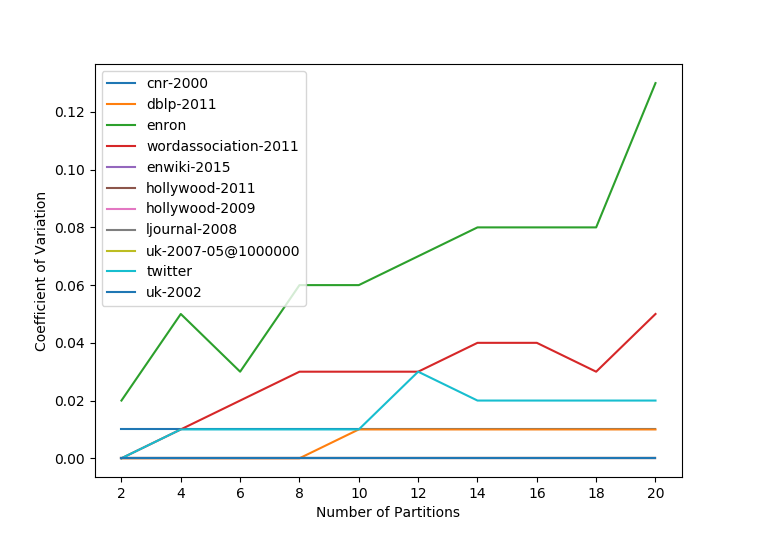
\includegraphics[width=\columnwidth]{../good_plots/range_as_cv_modulo.png}
	\caption{Range of the maximum number of edges handled by each worker to the 
		minimum handled by any worker, expressed by the coefficient of 
		variation, 
		for various numbers of partitions, with modulo partitioning.}
	\label{fig:cv_mod}
\end{figure}

\begin{figure}
	\centering
	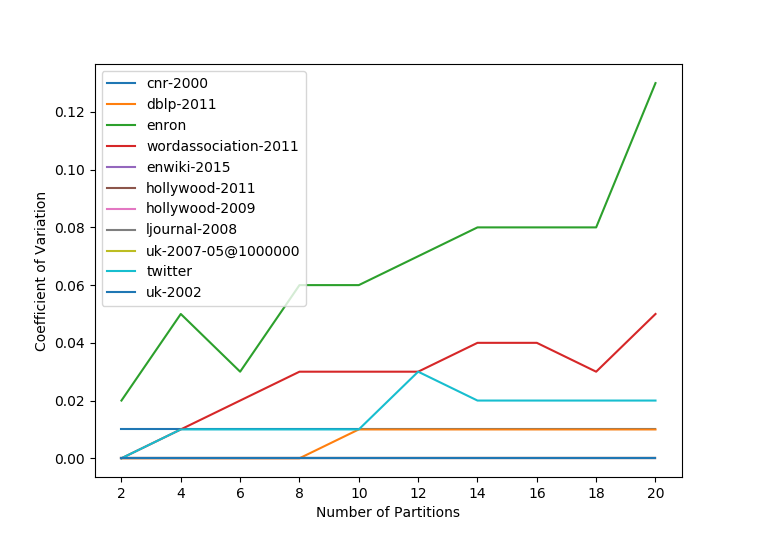
\includegraphics[width=\columnwidth]{../good_plots/range_as_cv_modulo.png}
	\caption{Range of the maximum number of edges handled by each worker to the 
		minimum handled by any worker, expressed by the coefficient of 
		variation, for various numbers of partitions, with segmented 
		partitioning.}
	\label{fig:cv_range}
\end{figure}



\subsection{Setting up Giraph}
1. Look at all the settings file and decribe important settings 


\subsubsection{Challenges for Beginner Giraph Users}

A significant amount of the time spent on this project was spent setting up our 
cluster and installing Giraph and all of its dependencies. Even for a 
well-supported and widely used piece of software like Giraph, this was a time 
consuming challenge. To begin with, version mismatches of Java, HDFS, Ubuntu, 
and Giraph itself caused a number of difficult-to-debug errors. For example, 
installing the most recent version of Java caused a mysterious build error that 
took hours to track down a workaround for (the workaround being to downgrade 
Java). Additionally, once Giraph had been successfully built, a total of eight 
hours was spent tuning various settings before the example job provided in the 
documentation would run without error. This was due to a number of factors. 
First, configuration settings are scattered across many different files, making 
it challenging to identify the source of a problem and difficult to predict how 
the settings would interact with each other. Second, few facilities existed for 
fine-tuning resource allocation. Many jobs failed with ``out of memory'' 
exceptions because it was difficult to tune the amount of memory they would be 
allocated. Third, error messages are not gathered in a central location - the 
existence of numerous log files made tracking down errors time consuming. 
Finally, Giraph seems to be a highly sensitive and delicate system. 
Unfortunately, as a result it is fragile: the slightest misallocation or 
imbalance of a resource causes jobs to fail with little explanation.

Our conclusion was that Giraph is a tool that is best used for large, 
heavy-duty workloads. For simple graph processing, one machine and writing 
one's own graph processing code may be the more straightforward solution. It 
seems likely that Giraph is in fact optimized for such workloads, given the 
difficulty we experienced in trying to make Giraph use ``small'' input graphs 
(less than a million 
nodes).

\subsection{Effect of different partition schemes}
